\section{Theoretical Motivation}

The field of nuclear and particle physics grew tremendously during the middle part of the 20th century.  As the Stanford Linear Accelerator (SLAC) accelerated electrons and collided them into various types of targets, previously unknown particles were discovered rapidly.  The abundance of particles was eventually explained by Gell-Man and Zweig with the inclusion of a set of new fundemental particles called quarks that carried a new degree of freedom known as color.  These ideas birthed the Quark Model which successfully predicted the masses and existence of new particles made of quarks, and eventually grew into Quantum Chromodynamics (QCD).  \\

A key feature of Quantum Chromodynamics is confinement; bound states of quarks must be colorless and quarks cannot be directly observed outside of the Hadrons they compose.  During the last 50 years, quark momenta within Hadrons has been studied successfully with collinear parton distribution functions (PDF's).  At leading order these functions $f(x)$ can be interpreted as the probability to find a quark with a colinear momentum fraction $x$ in a certain type of Hadron.  However, the one dimensional momentum distributions don't tell the full story of what's happening inside the Hadron.  During the last 15-20 years the focus has shifted to the study of 3-dimensional nucleon structure. \\

The transverse momentum dependent parton distribution functions (TMD's) are a set of functions $f(x, \vec{k}_{T})$ that describe quark distributions for a quark with momentum fraction $x$ and a momentum in the transverse plane $\vec{k}_{T}$.  TMD functions are expected to be universal, and show up in the cross sections for Drell-Yan (PP collisions) as well as Semi-Inclusive Deep Inelastic Scattering (SIDIS) events.  This thesis work will measure the latter.  

\subsection{Transeverse Momentum Dependent Parton Distribution Functions}

At leading order (twist), there are 8 TMD's each corresponding to different combinations of quark and nucleon spin.  They are shown in figure \ref{fig:tmd-table}.  The Boer-Mulders function $h^{1}_{\perp}$ for example, describes the difference in transverse quark polarization in an unpolarized nucleus, and has attracted a lot of interest for it's possible connection to quark angular momentum.  Performing different types of SIDIS and DY experiment gives access to different TMD functions.  

\begin{figure}
  \centering
  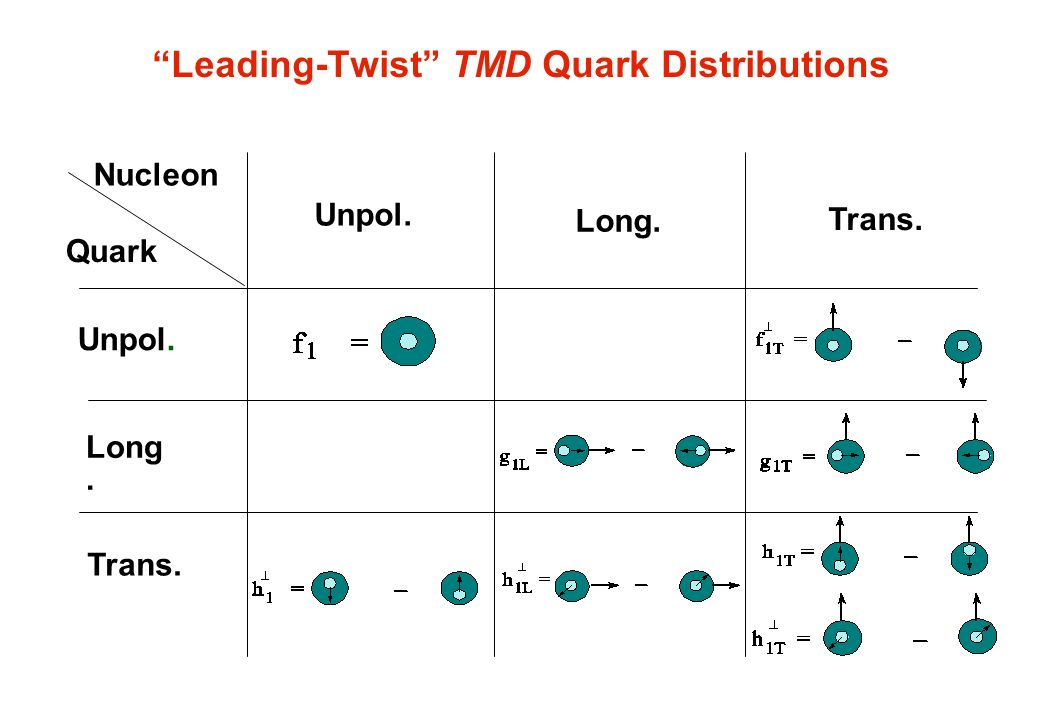
\includegraphics[width=10cm]{image/tmd-table.jpg}
  \caption{Shown above, the 8 leading twist TMD PDF's and thier interpretation in terms of different combinations of quark/nucleon spin.}
  \label{fig:tmd-table}
\end{figure}

\subsection{SIDIS Cross Section}
Deep Inelastic Scattering (DIS) events are those in which a lepton $e(l)$ collides with a hadron $h(P)$ (in our case a proton), transferring sufficient momentum $Q^{2} \geq 1.0 \: GeV^{2}/c^{2}$ to the hadron to interact with one of it's constituent partons.  An inclusive event is one in which only the outgoing lepton is identified and the kinematics are calculated based on the difference between the beam leptons and the final state lepton.  Semi-Inclusive DIS (SIDIS) events are those in which one (or more) hadron is detected in the final state along with the scattered lepton $e'(l')$.  

\begin{equation}
  e(l) + h(P) \rightarrow e'(l') + h(P_{h}) + X 
\end{equation}

In DIS and SIDIS it is customary to define the following kinematic variables (where $q = l - l'$ and $Q^{2} = -q^{2}$). 

\begin{figure}
  \centering
  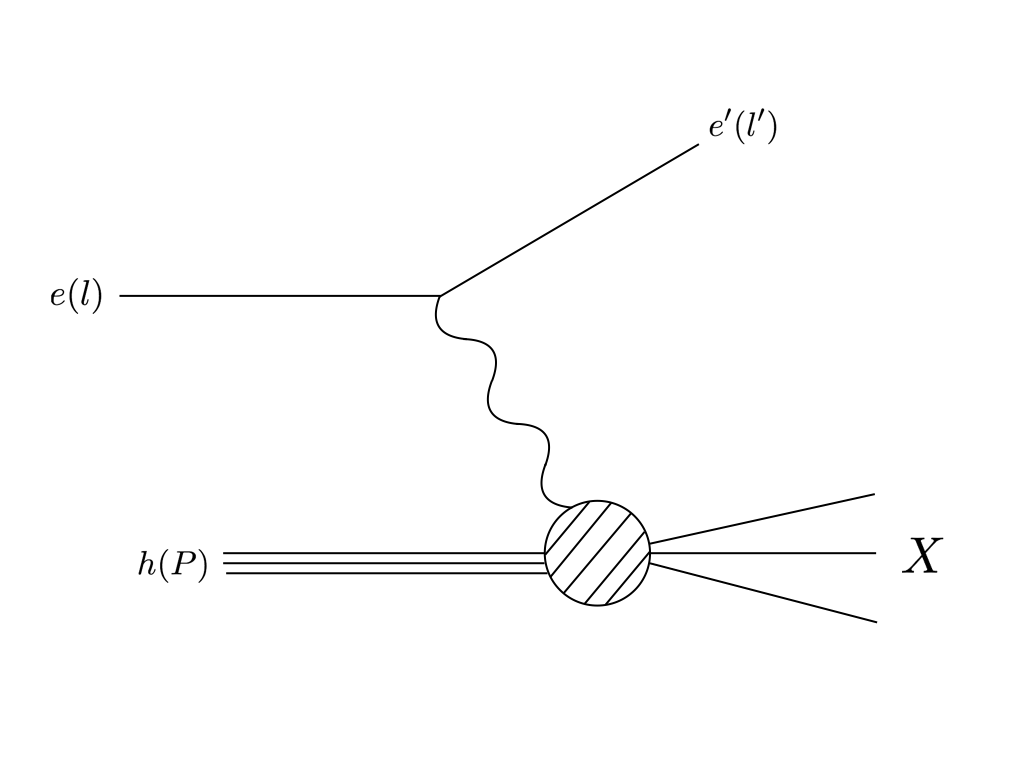
\includegraphics[width=10cm]{image/disFeynman.png}
  \label{fig:dis}
  \caption{ Inelastic lepton-hadron scattering, proceeding by exchange of a virtual Boson (photon in this dissertation). }
\end{figure}

\begin{align}
  x = \frac{Q^{2}}{2P \cdot q} && y = \frac{P \cdot q}{P \cdot l} && z = \frac{P \cdot P_{h}}{P \cdot q} && \gamma = \frac{2Mx}{Q}
\end{align}

The outgoing azimuthal angle of the hadron is defined by,

\begin{align}
  cos\phi_h = -\frac{l_\mu P_{h\nu} g^{\mu \nu}_{\perp}}{\sqrt{l^{2}_{\perp} P^{2}_{h\perp}}} &&
  sin\phi_h = -\frac{l_\mu P_{h\nu} \epsilon^{\mu \nu}_{\perp}}{\sqrt{l^{2}_{\perp} P^{2}_{h\perp}}} 
\end{align}

Where the transverse components of the electron and hadron momenta to the virtual photon have been defined $l_{\perp} = g^{\mu \nu}_{\perp} l_{\nu}$ and $P^{\mu}_{h\perp} = g^{\mu \nu}_{\perp}$.  The tensors are defined by,

\begin{gather}
  g^{\mu \nu}_{\perp} = g^{\mu \nu} - \frac{q^\mu P^\nu + P^\mu q^\nu}{P \cdot q (1 + \gamma^2)} + \frac{\gamma^{2}}{1 + \gamma^2} \left( \frac{q^\mu q^\nu}{Q^2} - \frac{P^\mu P^\nu}{M^2}\right) \\
  \epsilon^{\mu \nu}_{\perp} = \epsilon^{\mu \nu \rho \sigma} \frac{P_\rho q_\sigma}{P \cdot q \sqrt{1 + \gamma^2}}
\end{gather}
 
The differential cross section for SIDIS can be written as a contraction between two tensors, belonging to the leptonic and hadronic parts of the scattering.

\begin{equation}
  \frac{d\sigma}{dx_{B} dy dz_{h} dq_{T}^{2}} = \frac{\pi \alpha^{2}}{2 Q^{4}} L_{\mu \nu} 2M W^{\mu \nu}
\end{equation}

Where the leptonic tensor is calculated using standard trace techniques as,

\begin{equation}
  L_{\mu \nu} = \delta_{\lambda \lambda'} \left( 2 l_{\mu} l'_{\nu} + 2 l_{\nu} l'_{\mu} - Q^{2} g^{\mu \nu} + 2i\lambda \epsilon_{\mu \nu \sigma \tau} q^{\sigma} l^{\tau} \right) 
\end{equation}

here $\lambda$ refers to the electron helicity. The hadronic tensor is defined as,

\begin{gather}
  2MW^{\mu \nu} = \frac{1}{2\pi} \sum_{X} \int \frac{d^{3}P_{X}}{(2\pi)^{3}2P^{0}_{X}} (2\pi)^{4} \delta^{4} \left( q + P - P_{x} - P_{h} \right) \times
  \bra{P,S} J_{\mu}(0) \ket{P_{X}} \bra{P_{X}} J_{\nu}(0) \ket{P,S} \nonumber \\
  = \frac{1}{2\pi} \int d^{4}x e^{iq\cdot x} \bra{P,S} J_{\mu}(x) J_{\nu}(0) \ket{P,S}
  \label{eqn:hadronictensor}
\end{gather}

where $X$ contains all possible final state particles.  The differential cross section for SIDIS can be written in a model independent way by introducing a set of structure functions $F$,

\begin{eqnarray}
\frac{d\sigma^{e^-P\to e^-hX}}{dx_B \, dQ^{2} \,dz\, d\phi_h\, d p_{h\perp}^2}
&=&\frac{\alpha^2_{em}}{2x_B y Q^2}
\frac{y^2}{1-\varepsilon}  ( 1+\frac{\gamma^2}{2x_B} ) \Bigl\{  \nonumber \\
&& F_{UU ,T} +  \varepsilon F_{UU ,L}
+ \sqrt{2\,\varepsilon (1+\varepsilon)} \cos\phi_h F_{UU}^{\cos\phi_h}
+ \varepsilon \cos(2\phi_h) F_{UU}^{\cos 2\phi_h} \nonumber \\
&+& \lambda_e
\sqrt{2\,\varepsilon (1-\varepsilon)} \sin\phi_h F_{LU}^{\sin\phi_h}
+ \lambda \big[ \sqrt{2 \varepsilon (1+\varepsilon)} \sin\phi_h F_{UL}^{\sin\phi_h}
  +  \varepsilon \sin(2\phi_h) F_{UL}^{\sin 2\phi_h} \big] \nonumber \\
&+&  \lambda_e \lambda
\big[\sqrt{1-\varepsilon^2} F_{LL}
  +\sqrt{2\varepsilon (1-\varepsilon)} \cos\phi_h F_{LL}^{\cos \phi_h}\big] \nonumber \\
&+& s_\perp
\big[ \sin(\phi_h-\phi_S) \bigl(F_{UT ,T}^{\sin(\phi_h -\phi_S)}
  + \varepsilon\, F_{UT ,L}^{\sin(\phi_h -\phi_S)}\bigr) \nonumber \\
  && \phantom{s_\perp}
  + \varepsilon \sin(\phi_h+\phi_S) F_{UT}^{\sin(\phi_h +\phi_S)}
  + \varepsilon \sin(3\phi_h-\phi_S) F_{UT}^{\sin(3\phi_h -\phi_S)} \nonumber \\
  && \phantom{s_\perp}
  + \sqrt{2\,\varepsilon (1+\varepsilon)} \sin\phi_S F_{UT}^{\sin \phi_S }
  + \sqrt{2\,\varepsilon (1+\varepsilon)} \sin(2\phi_h-\phi_S) F_{UT}^{\sin(2\phi_h -\phi_S)}\big]\nonumber \\
&+& \lambda_e s_\perp
\big[\sqrt{1-\varepsilon^2} \cos(\phi_h-\phi_S) F_{LT}^{\cos(\phi_h -\phi_S)}
  +\sqrt{2\varepsilon (1-\varepsilon)} \cos\phi_S F_{LT}^{\cos \phi_S} \nonumber \\
  && \phantom{\lambda_e s_\perp}
  +\sqrt{2\,\varepsilon (1-\varepsilon)} \cos(2\phi_h-\phi_S) F_{LT}^{\cos(2\phi_h - \phi_S)} \big] \Bigr\},
\label{e:crossmaster}
\end{eqnarray}

which is presented in \cite{bacchetta, mulders}. For the unpolarized beam and target case we have,

\begin{eqnarray}
  \frac{d\sigma^{e^-P\to e^-hX}}{dx_B \, dQ^{2}\, dz\, d\phi_h\, d p_{h\perp}^2} = \frac{\alpha^2_{em}}{2x_B y Q^2} \frac{y^2}{1-\varepsilon}  ( 1+\frac{\gamma^2}{2x_B} ) \Bigl\{ F_{UU ,T} +  \varepsilon F_{UU ,L} \nonumber \\
  + \sqrt{2\,\varepsilon (1+\varepsilon)} \cos\phi_h F_{UU}^{\cos\phi_h}+ \varepsilon \cos(2\phi_h) F_{UU}^{\cos 2\phi_h} \Bigr\}
\end{eqnarray}

The unpolarized structure functions can be written as a convolution of $f_1$ TMD and $D_1$ Fragmentation Function.

\begin{equation}
  F_{UU,T} = x \sum_{a} e^{2}_{a} \int d^{2}\vec{p}_{\perp} d^{2}\vec{k}_{\perp} \delta^{(2)} \left( z\vec{k}_{\perp} + \vec{p}_{\perp} - \vec{P}_{h\perp} \right) f_{1}^{a}(x, \vec{k}_{\perp}^{2}) D_{1}^{a}(z, \vec{p}_{\perp}^{2})
\end{equation}


